\section{Span-Selection Baselines}
\label{app:select}

This appendix details the four span selectors compared in Section \ref{sec:predictfull} (scripts and full per-cell tables are released in the accompanying repository).

\subsection{Selector definitions}

\paragraph{Statistic predictor (ours).} The leave-one-dataset-out ridge predictor of Section \ref{sec:predictfull} ($k{=}3$ features selected inside each fold by $|\rho|$, predicting $\log_2 L^*$ and rounding to the nearest grid point), computed from train-split statistics. A single $n{=}28$ LOO regressor produces the predictions for both the sixteen main-suite cells and the pooled twenty-eight-cell view of Section \ref{sec:predictfull}; the two rows in Table \ref{tab:selectors} differ only in which cells they aggregate.

\paragraph{Validation selection (standard HPO).} For each run we parse the per-epoch validation loss (the early-stopping criterion) and take its minimum as that run's validation error; the selected lookback minimizes the seed-averaged validation error. All 32 dataset$\times$model rows (four families) parsed successfully. A per-seed variant (select per seed, then average) gives an almost identical mean regret ($+0.0036$ vs.\ $+0.0027$ MSE).

\paragraph{PACF last-significant-lag.} On the train split ($\le 32$ channels, seed-0 subsample), ACF (FFT, max lag 2880) is computed and Levinson--Durbin recursion yields the PACF; the suggested order is the largest lag outside the 95\% band, mapped to the nearest grid point on the $\log_2$ scale.

\paragraph{AIC order.} From the same recursion, the AR($p$) innovation variance gives $\mathrm{AIC}(p) = N \log \hat{\sigma}^2(p) + 2p$ (the Yule--Walker construction of R's \texttt{ar(aic=TRUE)}); the argmin order is mapped to the grid as above.

\subsection{Results on the trained matrix}

\begin{table}[t]
\caption{Selector comparison on the 16 dataset$\times$model cells of the main suite (8 datasets $\times$ \{iTransformer, DLinear\}): exact hits against the test oracle, mean absolute and relative test-MSE regret, and selection cost. Under the leakage-free train-split convention the statistic predictor no longer matches validation selection for trained models. PACF degenerates to always picking 2880; its six exact hits are exactly the cells right-censored at the scan ceiling, and its misses are catastrophic (exchange rate $+261\%$/$+489\%$ relative). Per-cell values are included in the released run ledger.}
\label{tab:selectors}
\centering\footnotesize
\begin{tabular}{lcccc l}
\toprule
Selector & Exact hit & Mean regret & Mean rel.\ & Median rel.\ & Cost \\
\midrule
Statistic predictor ($k{=}3$ LOO) & 3/16 & $+0.0075$ & $+4.52\%$ & $+2.30\%$ & $\approx 0$ (3 statistics) \\
Validation selection & \textbf{8/16} & \textbf{$+0.0031$} & \textbf{$+1.01\%$} & \textbf{$+0.07\%$} & 5 spans $\times$ full training \\
AIC order $\to$ grid & 2/16 & $+0.0080$ & $+3.49\%$ & $+2.91\%$ & low \\
PACF last sig.\ lag $\to$ grid & 6/16 (degenerate) & $+0.0786$ & $+57.8\%$ & $+10.09\%$ & low \\
\midrule
\multicolumn{6}{l}{\emph{Pooled extension suite (14 datasets $\times$ 2 families $=$ 28 cells)}} \\
Statistic predictor ($k{=}3$ LOO) & 8/28 & --- & $+5.33\%$ & $+2.30\%$ & $\approx 0$ \\
Validation selection & \textbf{16/28} & --- & \textbf{$+0.92\%$} & \textbf{$+0.00\%$} & 5 spans $\times$ full training \\
\bottomrule
\end{tabular}
\end{table}

Two distinct pools appear in this paper and should not be conflated: the \emph{pooled extension suite} above (fourteen datasets $\times$ two families, used for the headline comparison of Section \ref{sec:predictfull}), and the \emph{four-family main grid} (eight datasets $\times$ four model families $=$ 32 cells, all complete). Both statistic-predictor rows come from the same $n{=}28$ LOO regressor, so their difference reflects only the aggregated cells, not a refit. Validation selection on the four-family grid hits the oracle in 20/32 cells with mean relative regret $0.86\%$ (median $0.00\%$). Its failure modes are systematic: (a) long-window benefit that has not yet surfaced on the validation split (traffic/iTransformer: validation picks 720, oracle 2880, $+5.1\%$), (b) the symmetric short-window miss (ETTh2/PatchTST: validation picks 336, oracle 96, $+6.8\%$), and (c) weak resolution between adjacent grid points on ETT (ETTh1/iTransformer: validation picks 96 vs.\ oracle 720, $+2.0\%$).

\begin{table}[t]
\caption{PACF/AIC classical order selection: channel-median orders on level and first-differenced train series, mapped to the lookback grid, against the measured best lookback. PACF's significant lags extend to the 2880 cap on all eight datasets (a known long tail for strongly periodic series), so it always proposes 2880; AIC orders carry structure but measure only short-range linear predictability.}
\label{tab:pacf_aic}
\centering\footnotesize
\resizebox{\textwidth}{!}{%
\begin{tabular}{lcccc cc}
\toprule
Dataset & PACF order (level/diff) & $\to$ grid & AIC order (level/diff) & $\to$ grid & Best $L$ (iTr) & Best $L$ (DLin) \\
\midrule
ETTh1 & 2796 / 2812 & 2880 & 222 / 221 & 336 & 720 & 1440 \\
ETTh2 & 2766 / 2765 & 2880 & 266 / 265 & 336 & 96 & 720 \\
ETTm1 & 2874 / 2873 & 2880 & 598 / 675 & 720 & 336 & 336 \\
ETTm2 & 2876 / 2875 & 2880 & 677 / 676 & 720 & 336 & 2880 \\
Exchange & 2281 / 2445 & 2880 & 10 / 16 & 96 & 96 & 96 \\
Weather & 2872 / 2871 & 2880 & 169 / 297 & 96 / 336 & 336 & 2880 \\
Electricity & 2857 / 2857 & 2880 & 516 / 510 & 720 & 2880 & 2880 \\
Traffic & 2854 / 2856 & 2880 & 506 / 505 & 720 & 2880 & 2880 \\
\bottomrule
\end{tabular}}
\end{table}

\paragraph{Validation-window caveat.} In the standard TSLib protocol the number of validation windows varies with lookback, so each candidate's validation MSE is computed on a slightly different target set. We deliberately apply no correction for this: the variable-window validation set \emph{is} standard practice, and what we evaluate is that practice as-is. The per-seed selection variant changes the mean regret by only $0.0001$ MSE.

\subsection{Zero-shot selector (Chronos-Bolt)}

Chronos-Bolt has no training and no canonical validation usage, so we split the cached per-window test errors temporally: the first 50\% of windows serves as the selection set, the last 50\% as the evaluation set, at zero re-inference cost (electricity uses the stride-2 subsampled cache, internally fair across lookbacks).

\begin{table}[t]
\caption{Zero-shot span selection on Chronos-Bolt (evaluation on the temporally later 50\% of test windows). The dataset-level statistic rule (default 1440, veto to 96 when the dataset-mean drift index exceeds $0.6$) selects the \emph{same} lookback as validation selection on all eight datasets, at zero cost. Per-channel selection is worse than dataset-level selection on 2 of 4 datasets (selection noise), supporting that the exploitable gain lives at the dataset level.}
\label{tab:select_chronos}
\centering\footnotesize
\begin{tabular}{lccc ccc cc}
\toprule
Dataset & Val-sel.\ $L$ & Oracle $L$ & Hit & MSE (val-sel) & MSE (rule) & MSE (oracle) & Regret (val) & Regret (rule) \\
\midrule
ETTh1 & 1440 & 720 & n & 0.4205 & 0.4205 & 0.4192 & $+0.0013$ & $+0.0013$ \\
ETTh2 & 1440 & 1440 & Y & 0.3530 & 0.3530 & 0.3530 & $+0.0000$ & $+0.0000$ \\
ETTm1 & 1440 & 1440 & Y & 0.3549 & 0.3549 & 0.3549 & $+0.0000$ & $+0.0000$ \\
ETTm2 & 1440 & 1440 & Y & 0.2105 & 0.2105 & 0.2105 & $+0.0000$ & $+0.0000$ \\
Exchange & 96 & 96 & Y & 0.0949 & 0.0949 & 0.0949 & $+0.0000$ & $+0.0000$ \\
Weather & 1440 & 1440 & Y & 0.1474 & 0.1474 & 0.1474 & $+0.0000$ & $+0.0000$ \\
Electricity & 1440 & 720 & n & 0.1203 & 0.1203 & 0.1202 & $+0.0002$ & $+0.0002$ \\
Traffic & 1440 & 1440 & Y & 0.4178 & 0.4178 & 0.4178 & $+0.0000$ & $+0.0000$ \\
\bottomrule
\end{tabular}
\end{table}

The rule and validation selection coincide exactly on 8/8 datasets, and the two oracle misses are harmless (the zero-shot error surface is flat between 1440 and 720, $<0.4\%$). The coincidence is partly structural: the default 1440 arm is itself validation-optimal on six of the eight datasets, so the discriminative content of the rule is the exchange-rate veto, and the oracle comparison (two misses, both $<0.4\%$) bounds what either method leaves on the table. The veto threshold, however, sits in a dense region of ETT drift indices: on the train-split convention used by the budgeting chain, ETTh1 0.525, ETTh2 0.598, ETTm1 0.525, and ETTm2 0.599 all land just below the $0.6$ veto, while ETTh2's full-series value ($0.651$, Appendix \ref{app:stats}) would cross it. Every ETT dataset genuinely prefers 1440 in this zero-shot study, so the rule is correct on them either way; the threshold should nevertheless be read as illustrative rather than tuned.

\begin{figure}[t]
  \centering
  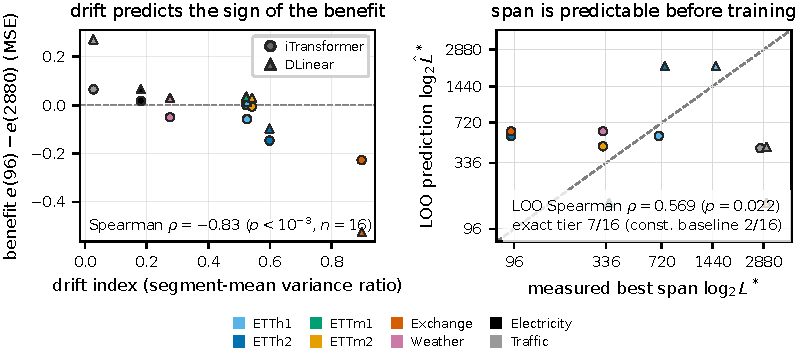
\includegraphics[width=0.52\linewidth]{figs/fig2_predictability.pdf}
  \caption{The effective span is predictable from training-free context statistics computed on the train split only. Left: drift index versus measured long-context benefit across the eight main-suite benchmarks and two model families (Spearman $\rho = -0.83$ over the sixteen samples; cluster-level reading over the eight datasets $\rho = -0.88$, $p = 0.004$). Right: leave-one-dataset-out predicted versus measured log-span (main-suite panel; the enlarged fourteen-dataset suite of Section \ref{sec:predictfull} gives $\rho = 0.63$; dashed line is identity).}
  \label{fig:predict}
\end{figure}

